% Options for packages loaded elsewhere
\PassOptionsToPackage{unicode}{hyperref}
\PassOptionsToPackage{hyphens}{url}
\documentclass[
]{article}
\usepackage{xcolor}
\usepackage[margin=1in]{geometry}
\usepackage{amsmath,amssymb}
\setcounter{secnumdepth}{-\maxdimen} % remove section numbering
\usepackage{iftex}
\ifPDFTeX
  \usepackage[T1]{fontenc}
  \usepackage[utf8]{inputenc}
  \usepackage{textcomp} % provide euro and other symbols
\else % if luatex or xetex
  \usepackage{unicode-math} % this also loads fontspec
  \defaultfontfeatures{Scale=MatchLowercase}
  \defaultfontfeatures[\rmfamily]{Ligatures=TeX,Scale=1}
\fi
\usepackage{lmodern}
\ifPDFTeX\else
  % xetex/luatex font selection
\fi
% Use upquote if available, for straight quotes in verbatim environments
\IfFileExists{upquote.sty}{\usepackage{upquote}}{}
\IfFileExists{microtype.sty}{% use microtype if available
  \usepackage[]{microtype}
  \UseMicrotypeSet[protrusion]{basicmath} % disable protrusion for tt fonts
}{}
\makeatletter
\@ifundefined{KOMAClassName}{% if non-KOMA class
  \IfFileExists{parskip.sty}{%
    \usepackage{parskip}
  }{% else
    \setlength{\parindent}{0pt}
    \setlength{\parskip}{6pt plus 2pt minus 1pt}}
}{% if KOMA class
  \KOMAoptions{parskip=half}}
\makeatother
\usepackage{color}
\usepackage{fancyvrb}
\newcommand{\VerbBar}{|}
\newcommand{\VERB}{\Verb[commandchars=\\\{\}]}
\DefineVerbatimEnvironment{Highlighting}{Verbatim}{commandchars=\\\{\}}
% Add ',fontsize=\small' for more characters per line
\usepackage{framed}
\definecolor{shadecolor}{RGB}{248,248,248}
\newenvironment{Shaded}{\begin{snugshade}}{\end{snugshade}}
\newcommand{\AlertTok}[1]{\textcolor[rgb]{0.94,0.16,0.16}{#1}}
\newcommand{\AnnotationTok}[1]{\textcolor[rgb]{0.56,0.35,0.01}{\textbf{\textit{#1}}}}
\newcommand{\AttributeTok}[1]{\textcolor[rgb]{0.13,0.29,0.53}{#1}}
\newcommand{\BaseNTok}[1]{\textcolor[rgb]{0.00,0.00,0.81}{#1}}
\newcommand{\BuiltInTok}[1]{#1}
\newcommand{\CharTok}[1]{\textcolor[rgb]{0.31,0.60,0.02}{#1}}
\newcommand{\CommentTok}[1]{\textcolor[rgb]{0.56,0.35,0.01}{\textit{#1}}}
\newcommand{\CommentVarTok}[1]{\textcolor[rgb]{0.56,0.35,0.01}{\textbf{\textit{#1}}}}
\newcommand{\ConstantTok}[1]{\textcolor[rgb]{0.56,0.35,0.01}{#1}}
\newcommand{\ControlFlowTok}[1]{\textcolor[rgb]{0.13,0.29,0.53}{\textbf{#1}}}
\newcommand{\DataTypeTok}[1]{\textcolor[rgb]{0.13,0.29,0.53}{#1}}
\newcommand{\DecValTok}[1]{\textcolor[rgb]{0.00,0.00,0.81}{#1}}
\newcommand{\DocumentationTok}[1]{\textcolor[rgb]{0.56,0.35,0.01}{\textbf{\textit{#1}}}}
\newcommand{\ErrorTok}[1]{\textcolor[rgb]{0.64,0.00,0.00}{\textbf{#1}}}
\newcommand{\ExtensionTok}[1]{#1}
\newcommand{\FloatTok}[1]{\textcolor[rgb]{0.00,0.00,0.81}{#1}}
\newcommand{\FunctionTok}[1]{\textcolor[rgb]{0.13,0.29,0.53}{\textbf{#1}}}
\newcommand{\ImportTok}[1]{#1}
\newcommand{\InformationTok}[1]{\textcolor[rgb]{0.56,0.35,0.01}{\textbf{\textit{#1}}}}
\newcommand{\KeywordTok}[1]{\textcolor[rgb]{0.13,0.29,0.53}{\textbf{#1}}}
\newcommand{\NormalTok}[1]{#1}
\newcommand{\OperatorTok}[1]{\textcolor[rgb]{0.81,0.36,0.00}{\textbf{#1}}}
\newcommand{\OtherTok}[1]{\textcolor[rgb]{0.56,0.35,0.01}{#1}}
\newcommand{\PreprocessorTok}[1]{\textcolor[rgb]{0.56,0.35,0.01}{\textit{#1}}}
\newcommand{\RegionMarkerTok}[1]{#1}
\newcommand{\SpecialCharTok}[1]{\textcolor[rgb]{0.81,0.36,0.00}{\textbf{#1}}}
\newcommand{\SpecialStringTok}[1]{\textcolor[rgb]{0.31,0.60,0.02}{#1}}
\newcommand{\StringTok}[1]{\textcolor[rgb]{0.31,0.60,0.02}{#1}}
\newcommand{\VariableTok}[1]{\textcolor[rgb]{0.00,0.00,0.00}{#1}}
\newcommand{\VerbatimStringTok}[1]{\textcolor[rgb]{0.31,0.60,0.02}{#1}}
\newcommand{\WarningTok}[1]{\textcolor[rgb]{0.56,0.35,0.01}{\textbf{\textit{#1}}}}
\usepackage{graphicx}
\makeatletter
\newsavebox\pandoc@box
\newcommand*\pandocbounded[1]{% scales image to fit in text height/width
  \sbox\pandoc@box{#1}%
  \Gscale@div\@tempa{\textheight}{\dimexpr\ht\pandoc@box+\dp\pandoc@box\relax}%
  \Gscale@div\@tempb{\linewidth}{\wd\pandoc@box}%
  \ifdim\@tempb\p@<\@tempa\p@\let\@tempa\@tempb\fi% select the smaller of both
  \ifdim\@tempa\p@<\p@\scalebox{\@tempa}{\usebox\pandoc@box}%
  \else\usebox{\pandoc@box}%
  \fi%
}
% Set default figure placement to htbp
\def\fps@figure{htbp}
\makeatother
\setlength{\emergencystretch}{3em} % prevent overfull lines
\providecommand{\tightlist}{%
  \setlength{\itemsep}{0pt}\setlength{\parskip}{0pt}}
\usepackage{hyperref}
\usepackage{amsmath}
\usepackage{amssymb}
\usepackage{graphicx}
\usepackage{fontspec}
\setmainfont{Cambria}
\setsansfont{Franklin Gothic Demi Cond}
\setmonofont{Courier New}
\usepackage[margin=1in]{geometry}
\usepackage{titlesec}
\titleformat{\section}{\Huge\bfseries\color{black}}{\thesection}{1em}{}
\titleformat{\subsection}{\huge\bfseries\color{black}}{\thesubsection}{1em}{}
\titleformat{\subsubsection}{\LARGE\bfseries\color{black}}{\thesubsubsection}{1em}{}
\usepackage{tocloft}
\renewcommand{\cftsecfont}{\small}
\renewcommand{\cftsubsecfont}{\footnotesize}
\renewcommand{\cftsecpagefont}{\small}
\renewcommand{\cftsubsecpagefont}{\footnotesize}
\renewcommand{\cftsecleader}{\cftdotfill{\cftdotsep}}
\usepackage{bookmark}
\IfFileExists{xurl.sty}{\usepackage{xurl}}{} % add URL line breaks if available
\urlstyle{same}
\hypersetup{
  hidelinks,
  pdfcreator={LaTeX via pandoc}}

\author{}
\date{\vspace{-2.5em}}

\begin{document}

\begin{titlepage}
    \begin{center}
        \textbf{\LARGE RÉPUBLIQUE DU SÉNÉGAL}\\[0.1cm]
        
\includegraphics[width=3cm]{"../Documents/Logo SEN.png"} \\[0.1cm]  
        \textbf{\large Un Peuple - Un But - Une Foi}\\[0.2cm]
        
        \textbf{\LARGE Ministère de l'Économie, du Plan et de la Coopération}\\[0.1cm]
        
\includegraphics[width=4cm]{"../Documents/Logo-MP.png"} \\[0.1cm] 
        
        \textbf{\large Agence Nationale de la Statistique et de la Démographie (ANSD)}\\[0.2cm]
        
        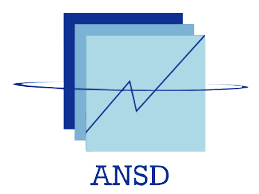
\includegraphics[width=4cm]{"../Documents/Logo-ANSD.png"} \\[0.1cm]  
        
        \textbf{\large École nationale de la Statistique et de l'Analyse économique Pierre Ndiaye (ENSAE)}\\[0.4cm]
        
\includegraphics[width=3cm]{"../Documents/ENSAE-Dakar-logo.png"} \\[0.1cm]
        
        \textbf{\LARGE PROJET STATISTIQUES SOUS R }\\[0.3cm]
        \textbf{\Huge \color{black} \textsf{TP8 : Cartographie sur R}}\\[0.2cm]
        \rule{\linewidth}{0.2mm} \\[0.5cm]
        
        \begin{minipage}{0.5\textwidth}
    \begin{flushleft} \large
        \emph{\textsf{Rédigé par :}}\\
        \textbf{KAFANDO G. Judicaël Oscar}\\
        \textbf{ILLY Jacques}\\
        \textit{Élèves ingénieurs statisticiens économistes}
    \end{flushleft}
\end{minipage}
        \hfill
        \begin{minipage}{0.4\textwidth}
            \begin{flushright} \large
                \emph{\textsf{Sous la supervision de :}} \\
                \textbf{M. Aboubacar HEMA}\\
                \textit{ANALYSTE DE RECHERCHE CHEZ IFPRI }
            \end{flushright}
        \end{minipage}

        \vfill

        {\large \textsf{Année scolaire : 2024-2025}}\\[0.5cm]
        
    \end{center}
\end{titlepage}

\newpage
\tableofcontents
\newpage

\section{\texorpdfstring{\textbf{Section 0 :
Généralité}}{Section 0 : Généralité}}\label{section-0-guxe9nuxe9ralituxe9}

\subsection{\texorpdfstring{\emph{1. Qu'est-ce que la Cartographie
?}}{1. Qu'est-ce que la Cartographie ?}}\label{quest-ce-que-la-cartographie}

La cartographie est une discipline essentielle qui permet de représenter
visuellement des données géographiques. Grâce à \textbf{R}, et notamment
aux bibliothèques comme \textbf{sf}, \textbf{ggplot2} et \textbf{tmap},
il est possible de charger, manipuler et visualiser des données
spatiales de manière efficace.

\subsection{\texorpdfstring{\emph{2. Qu'elle est l'usage de la
Cartographie
?}}{2. Qu'elle est l'usage de la Cartographie ?}}\label{quelle-est-lusage-de-la-cartographie}

La \textbf{cartographie} est largement utilisée dans de nombreux
domaines, notamment :\\
- L'urbanisme et l'aménagement du territoire\\
- Les sciences environnementales\\
- L'économie et la planification statistique\\
- La gestion des ressources naturelles

En utilisant \textbf{R}, nous pouvons intégrer des données spatiales et
produire des cartes dynamiques et interactives.

\subsection{\texorpdfstring{\emph{3. Comprendre les Fichiers
Shapefiles}}{3. Comprendre les Fichiers Shapefiles}}\label{comprendre-les-fichiers-shapefiles}

Un \textbf{Shapefile} est un format de données géospatiales largement
utilisé pour stocker des informations cartographiques vectorielles
(points, lignes, polygones). Il est souvent utilisé avec les
\textbf{Systèmes d'Information Géographique (SIG)} et est composé de
plusieurs fichiers associés.

Un shapefile comprend généralement les fichiers suivants :\\
- \textbf{.shp} : Contient la géométrie des objets (polygones, lignes,
points).\\
- \textbf{.shx} : Un index permettant d'accéder rapidement aux entités
géographiques.\\
- \textbf{.dbf} : Une base de données contenant les attributs des
entités géographiques (nom, population, superficie, etc.).\\
- \textbf{.prj} : Définit le système de projection et de coordonnées
utilisé.

Ces fichiers sont essentiels pour représenter et analyser des entités
spatiales.

\newpage

\section{\texorpdfstring{\textbf{Section 1 : Installation des packages
et
Importation}}{Section 1 : Installation des packages et Importation}}\label{section-1-installation-des-packages-et-importation}

\subsection{\texorpdfstring{\emph{Installation des packages
nécesssaires}}{Installation des packages nécesssaires}}\label{installation-des-packages-nuxe9cesssaires}

\begin{Shaded}
\begin{Highlighting}[]
\NormalTok{packages }\OtherTok{\textless{}{-}}  \FunctionTok{c}\NormalTok{(}\StringTok{"dplyr"}\NormalTok{,}\StringTok{"haven"}\NormalTok{,}\StringTok{"sf"}\NormalTok{,}\StringTok{"ggplot2"}\NormalTok{,}\StringTok{"tmap"}\NormalTok{)}

\ControlFlowTok{for}\NormalTok{ (package }\ControlFlowTok{in}\NormalTok{ packages) \{}
  \ControlFlowTok{if}\NormalTok{(}\SpecialCharTok{!}\FunctionTok{requireNamespace}\NormalTok{(package,}\AttributeTok{quietly =} \ConstantTok{TRUE}\NormalTok{))\{}
    \FunctionTok{install.packages}\NormalTok{(package)}
\NormalTok{  \}}
  \FunctionTok{library}\NormalTok{(package,}\AttributeTok{character.only =} \ConstantTok{TRUE}\NormalTok{)}
\NormalTok{\}}
\end{Highlighting}
\end{Shaded}

\subsection{\texorpdfstring{\emph{Importation des
bases}}{Importation des bases}}\label{importation-des-bases}

Pour cette partie, toute nos bases sont nommées de la sorte :
\emph{EHCVM\_HDX\_} suivie du nom du pays. Donc nous ferons une boucle
pour les chargé.

\begin{Shaded}
\begin{Highlighting}[]
\NormalTok{pays  }\OtherTok{\textless{}{-}}  \FunctionTok{c}\NormalTok{(}\StringTok{"Burkina"}\NormalTok{,}\StringTok{"Senegal"}\NormalTok{,}\StringTok{"Niger"}\NormalTok{,}\StringTok{"Benin"}\NormalTok{) }\CommentTok{\# Liste des pays}
\NormalTok{chemin\_base }\OtherTok{\textless{}{-}}  \StringTok{"../Data/Base/"} \CommentTok{\# Chemin menant aux différentes bases}

\ControlFlowTok{for}\NormalTok{ (p }\ControlFlowTok{in}\NormalTok{ pays) \{}
  
\NormalTok{  fichier }\OtherTok{\textless{}{-}} \FunctionTok{paste0}\NormalTok{(chemin\_base, }\StringTok{"EHCVM\_HDX\_"}\NormalTok{, p, }\StringTok{".dta"}\NormalTok{) }\DocumentationTok{\#\# Chemin d\textquotesingle{}acces à la base : concatener chaque element sans espace}
  
\NormalTok{  base }\OtherTok{\textless{}{-}}\NormalTok{ haven}\SpecialCharTok{::}\FunctionTok{read\_dta}\NormalTok{(fichier) }\CommentTok{\# Importation des bases}
  \FunctionTok{assign}\NormalTok{(}\FunctionTok{paste0}\NormalTok{(}\StringTok{"EHCVM\_"}\NormalTok{, p), labelled}\SpecialCharTok{::}\FunctionTok{to\_factor}\NormalTok{(base)) }\CommentTok{\# Labeliser chaque base et l\textquotesingle{}affecter à un objet du type "EHCVM\_nompays"}
  
\NormalTok{\}}
\end{Highlighting}
\end{Shaded}

\newpage

\section{\texorpdfstring{\textbf{Section 2 : Cartographie sur les
pays}}{Section 2 : Cartographie sur les pays}}\label{section-2-cartographie-sur-les-pays}

\emph{1. Importation du shapefile}

\begin{Shaded}
\begin{Highlighting}[]
\NormalTok{shp\_adm0\_AF }\OtherTok{\textless{}{-}}\NormalTok{ sf}\SpecialCharTok{::}\FunctionTok{st\_read}\NormalTok{(}\StringTok{"../Data/Shapefile/Pays/afr\_g2014\_2013\_0.shp"}\NormalTok{) }\DocumentationTok{\#\# Shapefile delimitant par pays de l\textquotesingle{}Afrique}
\end{Highlighting}
\end{Shaded}

\emph{2. Correction des noms des pays}

Certains pays comme la \textbf{Côte d'Ivoire} ont du mal à s'afficher du
fait de l'encodage. Le texte d'origine est encodé en UTF-8 (format
standard des caractères internationaux).On Convertit les caractères en
ASCII en remplaçant les accents et caractères spéciaux par leurs
équivalents.

\begin{Shaded}
\begin{Highlighting}[]
\NormalTok{shp\_adm0\_AF}\SpecialCharTok{$}\NormalTok{ADM0\_NAME }\OtherTok{\textless{}{-}} \FunctionTok{iconv}\NormalTok{(shp\_adm0\_AF}\SpecialCharTok{$}\NormalTok{ADM0\_NAME, }\AttributeTok{from =} \StringTok{"UTF{-}8"}\NormalTok{, }\AttributeTok{to =} \StringTok{"ASCII//TRANSLIT"}\NormalTok{) }\CommentTok{\# Convertit les texte en suppriment les caractères spéciaux et les accents}
\end{Highlighting}
\end{Shaded}

\emph{3. Traçons la carte}

Nous traçons la carte avec \textbf{ggplot2} en utilisant la fonction
\texttt{geom\_sf()}. Nous utilisons également la fonction
\texttt{geom\_text()} pour ajouter les noms des régions.

\begin{Shaded}
\begin{Highlighting}[]
\NormalTok{ggplot2}\SpecialCharTok{::}\FunctionTok{ggplot}\NormalTok{() }\SpecialCharTok{+}
  \FunctionTok{geom\_sf}\NormalTok{(}\AttributeTok{data =}\NormalTok{ shp\_adm0\_AF, }\AttributeTok{fill =} \StringTok{"lightgreen"}\NormalTok{, }\AttributeTok{color =} \StringTok{"black"}\NormalTok{) }\SpecialCharTok{+} \CommentTok{\# Tracer la carte}
  
  \CommentTok{\# Ajouter les labels des régions avec âge moyen}
  \FunctionTok{geom\_sf\_text}\NormalTok{(}\AttributeTok{data =}\NormalTok{ shp\_adm0\_AF, }
               \FunctionTok{aes}\NormalTok{(}\AttributeTok{label =}\NormalTok{ ADM0\_NAME), }\CommentTok{\# Afficher le nom de la région }
               \AttributeTok{size =} \DecValTok{2}\NormalTok{, }\AttributeTok{color =} \StringTok{"black"}\NormalTok{) }\SpecialCharTok{+}  \CommentTok{\# METTRE le nom en noir et taille 3}
  
  \CommentTok{\# Ajout d\textquotesingle{}un cthème minimal}
  \FunctionTok{theme\_minimal}\NormalTok{() }\SpecialCharTok{+} 
  
  \CommentTok{\# Ajouter les labels pour les axes et le titre}
  \FunctionTok{labs}\NormalTok{(}\AttributeTok{x =} \StringTok{"Longitude"}\NormalTok{, }\AttributeTok{y =} \StringTok{"Latitude"}\NormalTok{, }\AttributeTok{title =} \StringTok{"Carte de l\textquotesingle{}Afrique avec les pays"}\NormalTok{) }\SpecialCharTok{+}  
  
  \CommentTok{\# Centrer le titre et les labels des axes}
  \FunctionTok{theme}\NormalTok{(}\AttributeTok{plot.title =} \FunctionTok{element\_text}\NormalTok{(}\AttributeTok{hjust =} \FloatTok{0.5}\NormalTok{),  }\CommentTok{\# Centrer le titre}
        \AttributeTok{axis.title.x =} \FunctionTok{element\_text}\NormalTok{(}\AttributeTok{hjust =} \FloatTok{0.5}\NormalTok{),  }\CommentTok{\# Centrer le titre de l\textquotesingle{}axe X}
        \AttributeTok{axis.title.y =} \FunctionTok{element\_text}\NormalTok{(}\AttributeTok{hjust =} \FloatTok{0.5}\NormalTok{),  }\CommentTok{\# Centrer le titre de l\textquotesingle{}axe Y}
        \AttributeTok{panel.grid =} \FunctionTok{element\_blank}\NormalTok{())  }\CommentTok{\# Supprimer la grille de fond}
\end{Highlighting}
\end{Shaded}

\pandocbounded{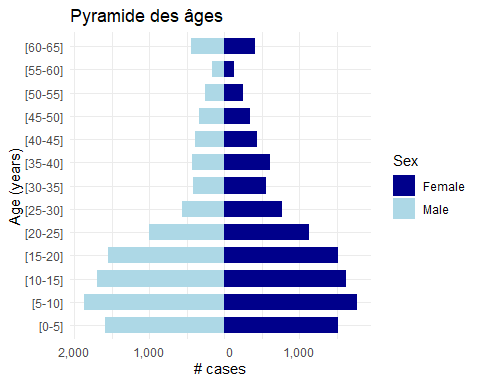
\includegraphics[keepaspectratio]{Stat_Desc_KAFANDO_ILLY_Syntaxe_TP8_files/figure-latex/unnamed-chunk-5-1.pdf}}

\newpage

\section{\texorpdfstring{\textbf{Section 3 : Cartographie par région sur
les
pays}}{Section 3 : Cartographie par région sur les pays}}\label{section-3-cartographie-par-ruxe9gion-sur-les-pays}

\subsection{\texorpdfstring{\emph{Importations des shapefiles
adéquats}}{Importations des shapefiles adéquats}}\label{importations-des-shapefiles-aduxe9quats}

Importons les fichiers de subdivision niveau régional

\begin{Shaded}
\begin{Highlighting}[]
\NormalTok{shp\_adm1\_BF }\OtherTok{\textless{}{-}}\NormalTok{ sf}\SpecialCharTok{::}\FunctionTok{st\_read}\NormalTok{(}\StringTok{"../Data/Shapefile/Region/bfa\_admbnda\_adm1\_igb\_20200323.shp"}\NormalTok{) }\DocumentationTok{\#\# Shapefile delimitant par région du Burkina}

\NormalTok{shp\_adm1\_SEN }\OtherTok{\textless{}{-}}\NormalTok{ sf}\SpecialCharTok{::}\FunctionTok{st\_read}\NormalTok{(}\StringTok{"../Data/Shapefile/Region/sen\_admbnda\_adm1\_anat\_20240520.shp"}\NormalTok{) }\DocumentationTok{\#\# Shapefile delimitant par région du Sénégal}

\NormalTok{shp\_adm1\_NER }\OtherTok{\textless{}{-}}\NormalTok{ sf}\SpecialCharTok{::}\FunctionTok{st\_read}\NormalTok{(}\StringTok{"../Data/Shapefile/Region/geoBoundaries{-}NER{-}ADM1.shp"}\NormalTok{) }\DocumentationTok{\#\# Shapefile delimitant par région du Niger}

\NormalTok{shp\_adm1\_BN }\OtherTok{\textless{}{-}}\NormalTok{ sf}\SpecialCharTok{::}\FunctionTok{st\_read}\NormalTok{(}\StringTok{"../Data/Shapefile/Region/geoBoundaries{-}BEN{-}ADM1.shp"}\NormalTok{) }\DocumentationTok{\#\# Shapefile delimitant par région du Bénin}
\end{Highlighting}
\end{Shaded}

\subsection{\texorpdfstring{\emph{Quelques
cartes}}{Quelques cartes}}\label{quelques-cartes}

\subsubsection{Cartes brutes}\label{cartes-brutes}

\textbf{1- Carte du Burkina avec les régions}

Nous traçons la carte avec \textbf{ggplot2} en utilisant la fonction
\texttt{geom\_sf()}. Nous utilisons également la fonction
\texttt{geom\_text()} pour ajouter les noms des régions.

\begin{Shaded}
\begin{Highlighting}[]
\NormalTok{ggplot2}\SpecialCharTok{::}\FunctionTok{ggplot}\NormalTok{() }\SpecialCharTok{+} 
  \FunctionTok{geom\_sf}\NormalTok{(}\AttributeTok{data =}\NormalTok{ shp\_adm1\_BF, }\AttributeTok{fill =} \StringTok{"lightyellow"}\NormalTok{, }\AttributeTok{color =} \StringTok{"black"}\NormalTok{) }\SpecialCharTok{+} \CommentTok{\# Tracer la carte avec un fond de couleur jaune clair et les tracé en noir}
  
  \CommentTok{\# Ajouter les labels des régions}
  \FunctionTok{geom\_sf\_text}\NormalTok{(}\AttributeTok{data =}\NormalTok{ shp\_adm1\_BF, }
               \FunctionTok{aes}\NormalTok{(}\AttributeTok{label =}\NormalTok{ ADM1\_FR), }\CommentTok{\# Afficher le nom de la région }
               \AttributeTok{size =} \DecValTok{3}\NormalTok{, }\AttributeTok{color =} \StringTok{"black"}\NormalTok{) }\SpecialCharTok{+}  \CommentTok{\# METTRE le nom en noir et taille 3}
  
  \CommentTok{\# Ajouter les labels pour les axes et le titre}
  \FunctionTok{labs}\NormalTok{(}\AttributeTok{x =} \StringTok{"Longitude"}\NormalTok{, }\AttributeTok{y =} \StringTok{"Latitude"}\NormalTok{, }\AttributeTok{title =} \StringTok{"Carte du Burkina suivant les régions"}\NormalTok{) }\SpecialCharTok{+}  
  
  \CommentTok{\# Centrer le titre et les labels des axes}
  \FunctionTok{theme}\NormalTok{(}\AttributeTok{plot.title =} \FunctionTok{element\_text}\NormalTok{(}\AttributeTok{hjust =} \FloatTok{0.5}\NormalTok{),  }\CommentTok{\# Centrer le titre de la carte}
        \AttributeTok{axis.title.x =} \FunctionTok{element\_text}\NormalTok{(}\AttributeTok{hjust =} \FloatTok{0.5}\NormalTok{),  }\CommentTok{\# Centrer le titre de l\textquotesingle{}axe X}
        \AttributeTok{axis.title.y =} \FunctionTok{element\_text}\NormalTok{(}\AttributeTok{hjust =} \FloatTok{0.5}\NormalTok{),  }\CommentTok{\# Centrer le titre de l\textquotesingle{}axe Y}
        \AttributeTok{panel.grid =} \FunctionTok{element\_blank}\NormalTok{())  }\CommentTok{\# Supprimer la grille de fond}
\end{Highlighting}
\end{Shaded}

\pandocbounded{\includegraphics[keepaspectratio]{Stat_Desc_KAFANDO_ILLY_Syntaxe_TP8_files/figure-latex/unnamed-chunk-7-1.pdf}}

\textbf{2- Carte du Bénin avec les régions}

Nous traçons la carte avec \textbf{ggplot2} en utilisant la fonction
\texttt{geom\_sf()}. Nous utilisons également la fonction
\texttt{geom\_text()} pour ajouter les noms des régions.

\begin{Shaded}
\begin{Highlighting}[]
\NormalTok{ggplot2}\SpecialCharTok{::}\FunctionTok{ggplot}\NormalTok{() }\SpecialCharTok{+}
  \FunctionTok{geom\_sf}\NormalTok{(}\AttributeTok{data =}\NormalTok{ shp\_adm1\_BN, }\AttributeTok{fill =} \StringTok{"gray"}\NormalTok{, }\AttributeTok{color =} \StringTok{"black"}\NormalTok{) }\SpecialCharTok{+} \CommentTok{\# Tracer la carte avec un fond de couleur gris  et les tracé en noir}
  
  \CommentTok{\# Ajouter les labels des régions }
  \FunctionTok{geom\_sf\_text}\NormalTok{(}\AttributeTok{data =}\NormalTok{ shp\_adm1\_BN, }
               \FunctionTok{aes}\NormalTok{(}\AttributeTok{label =}\NormalTok{ shapeName), }\CommentTok{\# Afficher le nom de la région }
               \AttributeTok{size =} \DecValTok{3}\NormalTok{, }\AttributeTok{color =} \StringTok{"black"}\NormalTok{) }\SpecialCharTok{+}  \CommentTok{\# METTRE le nom en noir et taille 3}
  
  \CommentTok{\#Ajouter un theme minimal}
  \FunctionTok{theme\_minimal}\NormalTok{() }\SpecialCharTok{+}
  
  \CommentTok{\# Ajouter les labels pour les axes et le titre}
  \FunctionTok{labs}\NormalTok{(}\AttributeTok{x =} \StringTok{"Longitude"}\NormalTok{, }\AttributeTok{y =} \StringTok{"Latitude"}\NormalTok{, }\AttributeTok{title =} \StringTok{"Carte du Bénin suivant les régions"}\NormalTok{) }\SpecialCharTok{+}  
  
  \CommentTok{\# Centrer le titre et les labels des axes}
  \FunctionTok{theme}\NormalTok{(}\AttributeTok{plot.title =} \FunctionTok{element\_text}\NormalTok{(}\AttributeTok{hjust =} \FloatTok{0.5}\NormalTok{),  }\CommentTok{\# Centrer le titre de la carte}
        \AttributeTok{axis.title.x =} \FunctionTok{element\_text}\NormalTok{(}\AttributeTok{hjust =} \FloatTok{0.5}\NormalTok{),  }\CommentTok{\# Centrer le titre de l\textquotesingle{}axe X}
        \AttributeTok{axis.title.y =} \FunctionTok{element\_text}\NormalTok{(}\AttributeTok{hjust =} \FloatTok{0.5}\NormalTok{),  }\CommentTok{\# Centrer le titre de l\textquotesingle{}axe Y}
        \AttributeTok{panel.grid =} \FunctionTok{element\_blank}\NormalTok{())  }\CommentTok{\# Supprimer la grille de fond}
\end{Highlighting}
\end{Shaded}

\pandocbounded{\includegraphics[keepaspectratio]{Stat_Desc_KAFANDO_ILLY_Syntaxe_TP8_files/figure-latex/unnamed-chunk-8-1.pdf}}

\subsection{Carte avec quelques statistiques par
région}\label{carte-avec-quelques-statistiques-par-ruxe9gion}

\textbf{Carte du Sénégal avec quelquesstatistiques par région}

Pour réussir une telle carte, nous avions besion non seulement de la
carte brute, mais aussi des statistiques concernées pour chaque région.

Calculons \emph{l'age moyen du chef de ménage} et le \emph{volume
horaire de travail moyen} pour chaque région

\begin{Shaded}
\begin{Highlighting}[]
\NormalTok{VolHor\_age\_moyen\_par\_region }\OtherTok{\textless{}{-}}\NormalTok{ EHCVM\_Senegal }\SpecialCharTok{\%\textgreater{}\%} \CommentTok{\# Précise la base de travail}
  \FunctionTok{group\_by}\NormalTok{(ADM1\_FR) }\SpecialCharTok{\%\textgreater{}\%} \CommentTok{\# Groupe suivant la région}
  \FunctionTok{summarise}\NormalTok{(}\AttributeTok{age\_moyen =} \FunctionTok{mean}\NormalTok{(age, }\AttributeTok{na.rm =} \ConstantTok{TRUE}\NormalTok{),}\CommentTok{\# calcule l\textquotesingle{}age moyen pour chaque région en ignorant les valeurs manquantes}
            \AttributeTok{volhor\_moyen =} \FunctionTok{mean}\NormalTok{(volhor, }\AttributeTok{na.rm =} \ConstantTok{TRUE}\NormalTok{)) }\SpecialCharTok{\%\textgreater{}\%} \CommentTok{\# calcule du volume horaire moyen pour chaque région en ignorant les valeurs manquantes}
  \FunctionTok{select}\NormalTok{(ADM1\_FR,volhor\_moyen,age\_moyen)}\CommentTok{\# Seléctionne le nom des regions, le volume horaire moyen et l\textquotesingle{}age moyen du chef de menage}

\NormalTok{VolHor\_age\_moyen\_par\_region }\CommentTok{\# affiche la base}
\end{Highlighting}
\end{Shaded}

\begin{verbatim}
## # A tibble: 14 x 3
##    ADM1_FR     volhor_moyen age_moyen
##    <chr>              <dbl>     <dbl>
##  1 Dakar              1776.      27.4
##  2 Diourbel           1148.      23.0
##  3 Fatick             1234.      24.1
##  4 Kaffrine           1159.      21.7
##  5 Kaolack            1242.      22.6
##  6 Kolda              1196.      22.0
##  7 Kédougou           1351.      22.1
##  8 Louga              1632.      22.5
##  9 Matam              1483.      22.8
## 10 Saint-Louis        1261.      22.9
## 11 Sédhiou            1390.      22.8
## 12 Tambacounda        1125.      21.6
## 13 Thiès              1368.      23.6
## 14 Ziguinchor         1721.      23.3
\end{verbatim}

Maintenant, nous associons l'âge moyen du CM et le volume horaire moyen
de travail au shapefile shp\_adm1\_SEN, en faisant correspondre par
région.

\begin{Shaded}
\begin{Highlighting}[]
\NormalTok{shp\_adm1\_SEN\_volhor\_age\_moyen }\OtherTok{\textless{}{-}} \FunctionTok{left\_join}\NormalTok{(shp\_adm1\_SEN,VolHor\_age\_moyen\_par\_region, }\AttributeTok{by =} \StringTok{"ADM1\_FR"}\NormalTok{) }\DocumentationTok{\#\# Jointure gauche en prenant comme identifiant ADM1\_FR}

\CommentTok{\#shp\_adm1\_SEN\_volhor\_age\_moyen}
\end{Highlighting}
\end{Shaded}

Nous traçons la carte maintenant.

\textbf{- Carte avec l'age moyen du chef de ménage}

\begin{Shaded}
\begin{Highlighting}[]
\NormalTok{ggplot2}\SpecialCharTok{::}\FunctionTok{ggplot}\NormalTok{(shp\_adm1\_SEN\_volhor\_age\_moyen) }\SpecialCharTok{+}
  \FunctionTok{geom\_sf}\NormalTok{( }\AttributeTok{fill =} \StringTok{"gray"}\NormalTok{, }\AttributeTok{color =} \StringTok{"black"}\NormalTok{) }\SpecialCharTok{+} \CommentTok{\# Tracer la carte en mettant le fond en gris}
  
  \CommentTok{\# Ajouter les labels des régions avec âge moyen}
  \FunctionTok{geom\_sf\_text}\NormalTok{( }
               \FunctionTok{aes}\NormalTok{(}\AttributeTok{label =} \FunctionTok{paste}\NormalTok{(ADM1\_FR, }\StringTok{"}\SpecialCharTok{\textbackslash{}n}\StringTok{"}\NormalTok{, }\FunctionTok{round}\NormalTok{(age\_moyen, }\DecValTok{0}\NormalTok{))), }\CommentTok{\# Afficher le nom de la région et la valeur de l\textquotesingle{}age moyen}
               \AttributeTok{size =} \DecValTok{3}\NormalTok{, }\AttributeTok{color =} \StringTok{"blue"}\NormalTok{) }\SpecialCharTok{+}  \CommentTok{\# Mettre le nom en blue et taille 3}
  
  \CommentTok{\#Ajouter theme minimal}
  \FunctionTok{theme\_minimal}\NormalTok{()}\SpecialCharTok{+}
  
  \CommentTok{\# Ajouter les labels pour les axes et le titre}
  \FunctionTok{labs}\NormalTok{(}\AttributeTok{x =} \StringTok{"Longitude"}\NormalTok{, }\AttributeTok{y =} \StringTok{"Latitude"}\NormalTok{, }\AttributeTok{title =} \StringTok{"Sénégal {-} Age moyen du CM par région"}\NormalTok{) }\SpecialCharTok{+}  
  
  \CommentTok{\# Centrer le titre et les labels des axes}
  \FunctionTok{theme}\NormalTok{(}\AttributeTok{plot.title =} \FunctionTok{element\_text}\NormalTok{(}\AttributeTok{hjust =} \FloatTok{0.5}\NormalTok{),  }\CommentTok{\# Centrer le titre}
        \AttributeTok{axis.title.x =} \FunctionTok{element\_text}\NormalTok{(}\AttributeTok{hjust =} \FloatTok{0.5}\NormalTok{),  }\CommentTok{\# Centrer le titre de l\textquotesingle{}axe X}
        \AttributeTok{axis.title.y =} \FunctionTok{element\_text}\NormalTok{(}\AttributeTok{hjust =} \FloatTok{0.5}\NormalTok{),  }\CommentTok{\# Centrer le titre de l\textquotesingle{}axe Y}
        \AttributeTok{panel.grid =} \FunctionTok{element\_blank}\NormalTok{())  }\CommentTok{\# Supprimer la grille de fond}
\end{Highlighting}
\end{Shaded}

\pandocbounded{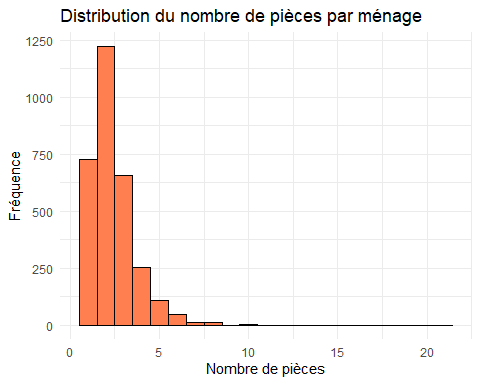
\includegraphics[keepaspectratio]{Stat_Desc_KAFANDO_ILLY_Syntaxe_TP8_files/figure-latex/unnamed-chunk-11-1.pdf}}

\textbf{- Carte avec le volume horaire de travail}

\begin{Shaded}
\begin{Highlighting}[]
\NormalTok{ggplot2}\SpecialCharTok{::}\FunctionTok{ggplot}\NormalTok{(shp\_adm1\_SEN\_volhor\_age\_moyen) }\SpecialCharTok{+}
  
  \FunctionTok{geom\_sf}\NormalTok{( }\FunctionTok{aes}\NormalTok{(}\AttributeTok{fill =}\NormalTok{ volhor\_moyen), }\AttributeTok{color =} \StringTok{"black"}\NormalTok{) }\SpecialCharTok{+} \CommentTok{\# Tracer la carte en mettant des couleurs pour chaque région  en fonction du volume horaire moyen}
  
  \FunctionTok{scale\_fill\_gradient}\NormalTok{(}\AttributeTok{low =} \StringTok{"lightgreen"}\NormalTok{, }\AttributeTok{high =} \StringTok{"darkgreen"}\NormalTok{, }\AttributeTok{name =} \StringTok{"Volume horaire moyen"}\NormalTok{) }\SpecialCharTok{+}  \CommentTok{\# Ajouter une palette de couleurs dégradé du bleu clair au bleu foncé  pour le volume horaire}
  
  
  \CommentTok{\# Ajouter les labels des régions avec âge moyen}
  \FunctionTok{geom\_sf\_text}\NormalTok{( }\FunctionTok{aes}\NormalTok{(}\AttributeTok{label =}\NormalTok{ ADM1\_FR), }\CommentTok{\# Afficher le nom de la région }
               \AttributeTok{size =} \DecValTok{3}\NormalTok{, }\AttributeTok{color =} \StringTok{"red"}\NormalTok{) }\SpecialCharTok{+}  \CommentTok{\# Mettre le nom en en rouge}
  
  \CommentTok{\#Ajouter theme minimal}
  \FunctionTok{theme\_minimal}\NormalTok{()}\SpecialCharTok{+}
  
  \CommentTok{\# Ajouter les labels pour les axes et le titre}
  \FunctionTok{labs}\NormalTok{(}\AttributeTok{x =} \StringTok{"Longitude"}\NormalTok{, }\AttributeTok{y =} \StringTok{"Latitude"}\NormalTok{, }\AttributeTok{title =} \StringTok{"Sénégal {-} Volume horaire moyen par région"}\NormalTok{) }\SpecialCharTok{+}  
  
  \CommentTok{\# Centrer le titre et les labels des axes}
  \FunctionTok{theme}\NormalTok{(}\AttributeTok{plot.title =} \FunctionTok{element\_text}\NormalTok{(}\AttributeTok{hjust =} \FloatTok{0.5}\NormalTok{),  }\CommentTok{\# Centrer le titre}
        \AttributeTok{axis.title.x =} \FunctionTok{element\_text}\NormalTok{(}\AttributeTok{hjust =} \FloatTok{0.5}\NormalTok{),  }\CommentTok{\# Centrer le titre de l\textquotesingle{}axe X}
        \AttributeTok{axis.title.y =} \FunctionTok{element\_text}\NormalTok{(}\AttributeTok{hjust =} \FloatTok{0.5}\NormalTok{),  }\CommentTok{\# Centrer le titre de l\textquotesingle{}axe Y}
        \AttributeTok{panel.grid =} \FunctionTok{element\_blank}\NormalTok{())  }\CommentTok{\# Supprimer la grille de fond}
\end{Highlighting}
\end{Shaded}

\pandocbounded{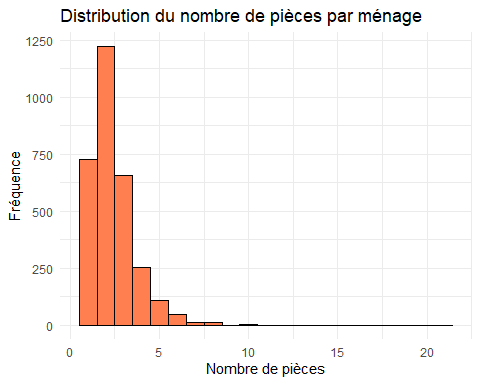
\includegraphics[keepaspectratio]{Stat_Desc_KAFANDO_ILLY_Syntaxe_TP8_files/figure-latex/unnamed-chunk-12-1.pdf}}

\newpage

\section{\texorpdfstring{\textbf{Section 4 : Cartographie par
département sur les
pays}}{Section 4 : Cartographie par département sur les pays}}\label{section-4-cartographie-par-duxe9partement-sur-les-pays}

\subsection{\texorpdfstring{\emph{Importations des shapefiles
adéquats}}{Importations des shapefiles adéquats}}\label{importations-des-shapefiles-aduxe9quats-1}

Importons les fichiers de subdivision niveau départemental
(\textbf{deuxième niveau de division}) .

\begin{Shaded}
\begin{Highlighting}[]
\NormalTok{shp\_adm2\_BF }\OtherTok{\textless{}{-}}\NormalTok{ sf}\SpecialCharTok{::}\FunctionTok{st\_read}\NormalTok{(}\StringTok{"../Data/Shapefile/Departement/bfa\_admbnda\_adm2\_igb\_20200323.shp"}\NormalTok{) }\DocumentationTok{\#\# Shapefile delimitant par département du Burkina}

\NormalTok{shp\_adm2\_SEN }\OtherTok{\textless{}{-}}\NormalTok{ sf}\SpecialCharTok{::}\FunctionTok{st\_read}\NormalTok{(}\StringTok{"../Data/Shapefile/Departement/sen\_admbnda\_adm2\_anat\_20240520.shp"}\NormalTok{) }\DocumentationTok{\#\# Shapefile delimitant par département du Sénégal}

\NormalTok{shp\_adm2\_NER }\OtherTok{\textless{}{-}}\NormalTok{ sf}\SpecialCharTok{::}\FunctionTok{st\_read}\NormalTok{(}\StringTok{"../Data/Shapefile/Departement/geoBoundaries{-}NER{-}ADM2.shp"}\NormalTok{) }\DocumentationTok{\#\# Shapefile delimitant par département du Niger}

\NormalTok{shp\_adm2\_BN }\OtherTok{\textless{}{-}}\NormalTok{ sf}\SpecialCharTok{::}\FunctionTok{st\_read}\NormalTok{(}\StringTok{"../Data/Shapefile/Departement/geoBoundaries{-}BEN{-}ADM2.shp"}\NormalTok{) }\DocumentationTok{\#\# Shapefile delimitant par département du Bénin}
\end{Highlighting}
\end{Shaded}

\subsection{\texorpdfstring{\emph{Quelques
cartes}}{Quelques cartes}}\label{quelques-cartes-1}

\subsubsection{Cartes brutes}\label{cartes-brutes-1}

\textbf{1- Carte du Niger avec les départements}

Nous traçons la carte avec \textbf{ggplot2} en utilisant la fonction
\texttt{geom\_sf()}. Nous utilisons également la fonction
\texttt{geom\_text()} pour ajouter les noms des départements.

\begin{Shaded}
\begin{Highlighting}[]
\NormalTok{ggplot2}\SpecialCharTok{::}\FunctionTok{ggplot}\NormalTok{() }\SpecialCharTok{+}
  \FunctionTok{geom\_sf}\NormalTok{(}\AttributeTok{data =}\NormalTok{ shp\_adm2\_NER, }\AttributeTok{fill =} \StringTok{"lightblue"}\NormalTok{, }\AttributeTok{color =} \StringTok{"black"}\NormalTok{) }\SpecialCharTok{+} \CommentTok{\# Tracer la carte en mettant un fond bleu et les tracés en noir}
  
  \CommentTok{\# Ajouter les labels des départements }
  \FunctionTok{geom\_sf\_text}\NormalTok{(}\AttributeTok{data =}\NormalTok{ shp\_adm2\_NER, }
               \FunctionTok{aes}\NormalTok{(}\AttributeTok{label =}\NormalTok{ shapeName), }\CommentTok{\# Afficher le nom du département }
               \AttributeTok{size =} \DecValTok{2}\NormalTok{, }\AttributeTok{color =} \StringTok{"black"}\NormalTok{) }\SpecialCharTok{+}  \CommentTok{\# Mettre le nom en noir et taille 2}
  
  \CommentTok{\# Ajouter les labels pour les axes et le titre}
  \FunctionTok{labs}\NormalTok{(}\AttributeTok{x =} \StringTok{"Longitude"}\NormalTok{, }\AttributeTok{y =} \StringTok{"Latitude"}\NormalTok{, }\AttributeTok{title =} \StringTok{"Carte du Niger suivant les départements"}\NormalTok{) }\SpecialCharTok{+}  
  
  \CommentTok{\# Centrer le titre et les labels des axes}
  \FunctionTok{theme}\NormalTok{(}\AttributeTok{plot.title =} \FunctionTok{element\_text}\NormalTok{(}\AttributeTok{hjust =} \FloatTok{0.5}\NormalTok{),  }\CommentTok{\# Centrer le titre de la carte}
        \AttributeTok{axis.title.x =} \FunctionTok{element\_text}\NormalTok{(}\AttributeTok{hjust =} \FloatTok{0.5}\NormalTok{),  }\CommentTok{\# Centrer le titre de l\textquotesingle{}axe X}
        \AttributeTok{axis.title.y =} \FunctionTok{element\_text}\NormalTok{(}\AttributeTok{hjust =} \FloatTok{0.5}\NormalTok{),  }\CommentTok{\# Centrer le titre de l\textquotesingle{}axe Y}
        \AttributeTok{panel.grid =} \FunctionTok{element\_blank}\NormalTok{())  }\CommentTok{\# Supprimer la grille de fond}
\end{Highlighting}
\end{Shaded}

\pandocbounded{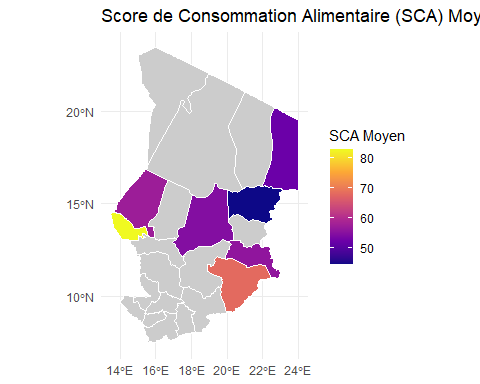
\includegraphics[keepaspectratio]{Stat_Desc_KAFANDO_ILLY_Syntaxe_TP8_files/figure-latex/unnamed-chunk-14-1.pdf}}

\textbf{2- Carte du Burkina avec les départements}

Nous traçons la carte avec \textbf{ggplot2} en utilisant la fonction
\texttt{geom\_sf()}. Nous utilisons également la fonction
\texttt{geom\_text()} pour ajouter les noms des départements.

\begin{Shaded}
\begin{Highlighting}[]
\NormalTok{ggplot2}\SpecialCharTok{::}\FunctionTok{ggplot}\NormalTok{() }\SpecialCharTok{+}
  \FunctionTok{geom\_sf}\NormalTok{(}\AttributeTok{data =}\NormalTok{ shp\_adm2\_BF, }\AttributeTok{fill =} \StringTok{"lightgreen"}\NormalTok{, }\AttributeTok{color =} \StringTok{"gray"}\NormalTok{) }\SpecialCharTok{+} \CommentTok{\# Tracer la carte avec un fond vert et des tracé en gris}
  
  \CommentTok{\# Ajouter les labels des départements}
  \FunctionTok{geom\_sf\_text}\NormalTok{(}\AttributeTok{data =}\NormalTok{ shp\_adm2\_BF, }
               \FunctionTok{aes}\NormalTok{(}\AttributeTok{label =}\NormalTok{ ADM2\_FR), }\CommentTok{\# Afficher le nom du département }
               \AttributeTok{size =} \DecValTok{2}\NormalTok{, }\AttributeTok{color =} \StringTok{"black"}\NormalTok{) }\SpecialCharTok{+}  \CommentTok{\# Mettre le nom en noir et taille 2}
  
  \CommentTok{\#Ajouter un theme }
  \FunctionTok{theme\_linedraw}\NormalTok{() }\SpecialCharTok{+}
  
  \CommentTok{\# Ajouter les labels pour les axes et le titre}
  \FunctionTok{labs}\NormalTok{(}\AttributeTok{x =} \StringTok{"Longitude"}\NormalTok{, }\AttributeTok{y =} \StringTok{"Latitude"}\NormalTok{, }\AttributeTok{title =} \StringTok{"Carte du Burkina suivant les provinces"}\NormalTok{) }\SpecialCharTok{+}  
  
  \CommentTok{\# Centrer le titre et les labels des axes}
  \FunctionTok{theme}\NormalTok{(}\AttributeTok{plot.title =} \FunctionTok{element\_text}\NormalTok{(}\AttributeTok{hjust =} \FloatTok{0.5}\NormalTok{),  }\CommentTok{\# Centrer le titre}
        \AttributeTok{axis.title.x =} \FunctionTok{element\_text}\NormalTok{(}\AttributeTok{hjust =} \FloatTok{0.5}\NormalTok{),  }\CommentTok{\# Centrer le titre de l\textquotesingle{}axe X}
        \AttributeTok{axis.title.y =} \FunctionTok{element\_text}\NormalTok{(}\AttributeTok{hjust =} \FloatTok{0.5}\NormalTok{),  }\CommentTok{\# Centrer le titre de l\textquotesingle{}axe Y}
        \AttributeTok{panel.grid =} \FunctionTok{element\_blank}\NormalTok{())  }\CommentTok{\# Supprimer la grille de fond}
\end{Highlighting}
\end{Shaded}

\pandocbounded{\includegraphics[keepaspectratio]{Stat_Desc_KAFANDO_ILLY_Syntaxe_TP8_files/figure-latex/unnamed-chunk-15-1.pdf}}

\subsubsection{Carte avec quelques
statistiques}\label{carte-avec-quelques-statistiques}

\textbf{1- Carte du Sénégal avec quelques statistiques par département}

Pour réussir une telle carte, nous avions besion non seulement de la
carte brute, mais aussi des statistiques concernées pour chaque
département.

Calculons \emph{l'age moyen au mariage} et le \emph{salaire moyen} moyen
pour chaque région

\begin{Shaded}
\begin{Highlighting}[]
\NormalTok{Base }\OtherTok{\textless{}{-}}\NormalTok{ EHCVM\_Senegal }\SpecialCharTok{\%\textgreater{}\%} \CommentTok{\# Precise la base de travail}
  
  \FunctionTok{group\_by}\NormalTok{(ADM2\_FR) }\SpecialCharTok{\%\textgreater{}\%} \CommentTok{\# Groupe suivant le departement}
  
  \FunctionTok{summarise}\NormalTok{(}\AttributeTok{salaire\_moyen =} \FunctionTok{mean}\NormalTok{(salaire, }\AttributeTok{na.rm =} \ConstantTok{TRUE}\NormalTok{), }\CommentTok{\# Calcul du salaire moyen par departement en ignorant les valeurs manquantes}
            
            \AttributeTok{agemar\_moyen =} \FunctionTok{mean}\NormalTok{(agemar, }\AttributeTok{na.rm =} \ConstantTok{TRUE}\NormalTok{)) }\SpecialCharTok{\%\textgreater{}\%} \CommentTok{\# calcule de l\textquotesingle{}age moyen au mariage pour chaque departement en ignorant les valeurs manquantes }
  
  \FunctionTok{select}\NormalTok{(ADM2\_FR,agemar\_moyen, salaire\_moyen)}\CommentTok{\# Seléctionne le nom des departement, l\textquotesingle{}age moyen au mariage   et le salaire moyen}

\NormalTok{Base }\CommentTok{\# afficher la base}
\end{Highlighting}
\end{Shaded}

\begin{verbatim}
## # A tibble: 39 x 3
##    ADM2_FR     agemar_moyen salaire_moyen
##    <chr>              <dbl>         <dbl>
##  1 Bambey              20.1       978657.
##  2 Bignona             24.1      1194895.
##  3 Birkelane           21.0      2897292.
##  4 Bounkiling          21.7      1347072 
##  5 Dagana              18.3       574863.
##  6 Dakar               24.4      1809377.
##  7 Fatick              23.1       847009.
##  8 Foundiougne         22.1       702762.
##  9 Gossas              21.7      1000656.
## 10 Goudiry             20.8       417907.
## # i 29 more rows
\end{verbatim}

Maintenant, nous associons l'âge moyen au mariage et le salaire moyen au
shapefile shp\_adm1\_SEN, en faisant correspondre par département.

\begin{Shaded}
\begin{Highlighting}[]
\NormalTok{shp\_adm2\_SEN\_Base }\OtherTok{\textless{}{-}} \FunctionTok{left\_join}\NormalTok{(shp\_adm2\_SEN,Base, }\AttributeTok{by =} \StringTok{"ADM2\_FR"}\NormalTok{) }\DocumentationTok{\#\# Jointure gauche en prenant comme identifiant ADM2\_FR}

\CommentTok{\#shp\_adm2\_SEN\_Base}
\end{Highlighting}
\end{Shaded}

Nous traçons la carte maintenant.

\textbf{- Carte avec le salaire moyen}

\begin{Shaded}
\begin{Highlighting}[]
\NormalTok{ggplot2}\SpecialCharTok{::}\FunctionTok{ggplot}\NormalTok{(shp\_adm2\_SEN\_Base) }\SpecialCharTok{+}
  \FunctionTok{geom\_sf}\NormalTok{( }\FunctionTok{aes}\NormalTok{(}\AttributeTok{fill =}\NormalTok{ salaire\_moyen), }\AttributeTok{color =} \StringTok{"black"}\NormalTok{) }\SpecialCharTok{+} \CommentTok{\# Tracer la carte en mettant les couleurs de chaque département en fonction du salaire moyen}
  \FunctionTok{scale\_fill\_gradient}\NormalTok{(}
    \AttributeTok{low =} \StringTok{"orange"}\NormalTok{, }\AttributeTok{high =} \StringTok{"darkred"}\NormalTok{,   }\CommentTok{\# Dégradé de orange au rouge}
    \AttributeTok{name =} \StringTok{"Salaire Moyen (FCFA)"}      \CommentTok{\# Nom de la légende}
\NormalTok{  ) }\SpecialCharTok{+}
  
  \CommentTok{\# Ajouter les labels des département}
  \FunctionTok{geom\_sf\_text}\NormalTok{( }
               \FunctionTok{aes}\NormalTok{(}\AttributeTok{label =}\NormalTok{ ADM2\_FR), }\CommentTok{\# Afficher le nom  }
               \AttributeTok{size =} \DecValTok{2}\NormalTok{, }\AttributeTok{color =} \StringTok{"black"}\NormalTok{) }\SpecialCharTok{+}  \CommentTok{\# Mettre le nom en noir}
  
  \CommentTok{\#Ajouter theme  (cadre)}
  \FunctionTok{theme\_linedraw}\NormalTok{()}\SpecialCharTok{+}
  
  \CommentTok{\# Ajouter les labels pour les axes et le titre}
  \FunctionTok{labs}\NormalTok{(}\AttributeTok{x =} \StringTok{"Longitude"}\NormalTok{, }\AttributeTok{y =} \StringTok{"Latitude"}\NormalTok{, }\AttributeTok{title =} \StringTok{"Sénégal {-} Volume horaire moyen du CM par département"}\NormalTok{) }\SpecialCharTok{+}  
  
  \CommentTok{\# Centrer le titre et les labels des axes}
  \FunctionTok{theme}\NormalTok{(}\AttributeTok{plot.title =} \FunctionTok{element\_text}\NormalTok{(}\AttributeTok{hjust =} \FloatTok{0.5}\NormalTok{),  }\CommentTok{\# Centrer le titre}
        \AttributeTok{axis.title.x =} \FunctionTok{element\_text}\NormalTok{(}\AttributeTok{hjust =} \FloatTok{0.5}\NormalTok{),  }\CommentTok{\# Centrer le titre de l\textquotesingle{}axe X}
        \AttributeTok{axis.title.y =} \FunctionTok{element\_text}\NormalTok{(}\AttributeTok{hjust =} \FloatTok{0.5}\NormalTok{),  }\CommentTok{\# Centrer le titre de l\textquotesingle{}axe Y}
        \AttributeTok{panel.grid =} \FunctionTok{element\_blank}\NormalTok{())  }\CommentTok{\# Supprimer la grille de fond}
\end{Highlighting}
\end{Shaded}

\pandocbounded{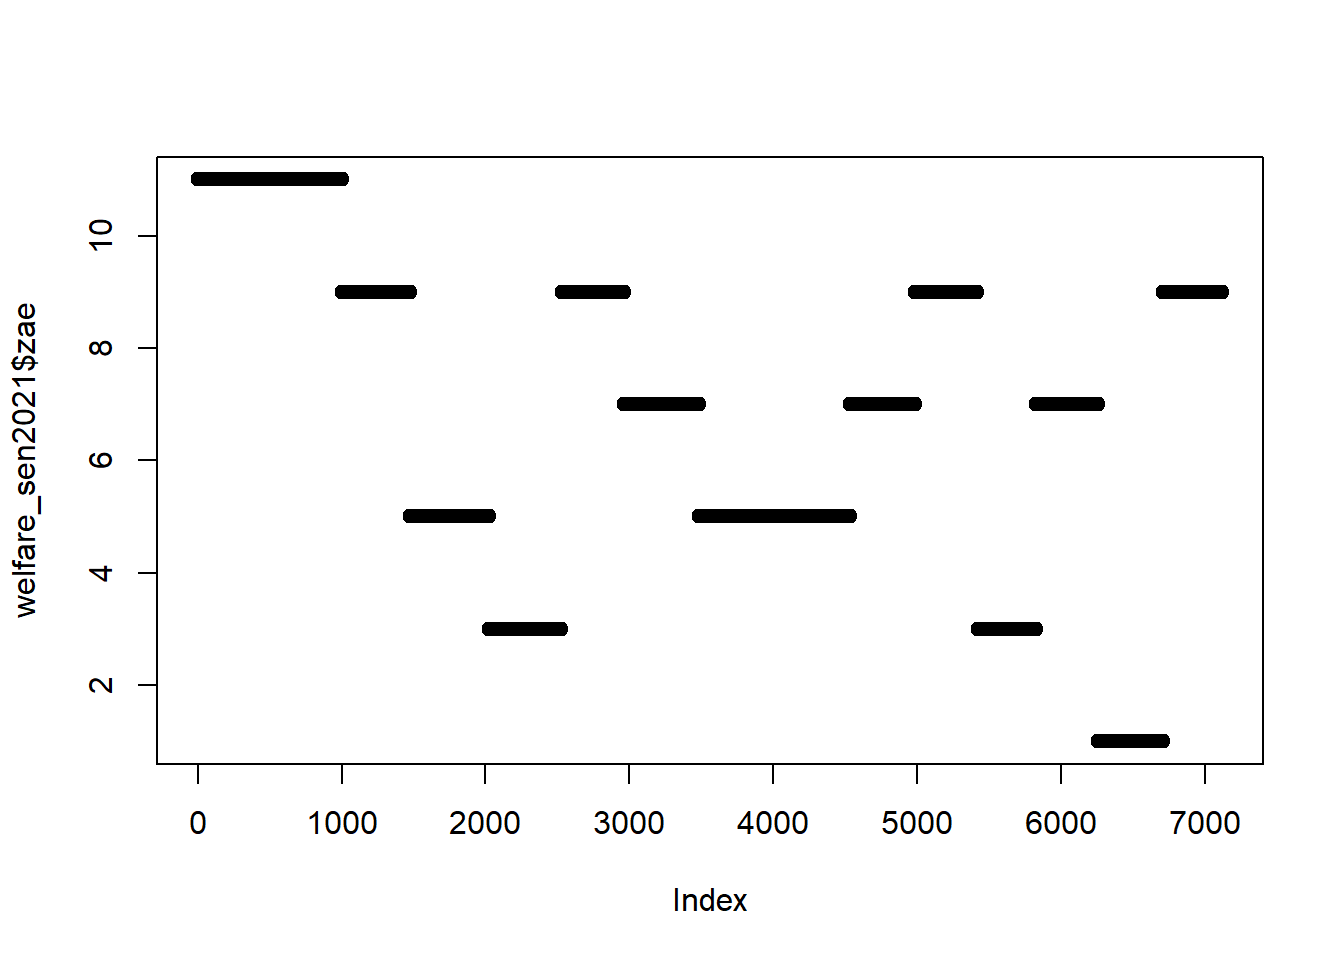
\includegraphics[keepaspectratio]{Stat_Desc_KAFANDO_ILLY_Syntaxe_TP8_files/figure-latex/unnamed-chunk-18-1.pdf}}

On constate que certains départements comme \emph{Médina-Yorofoula,
Sédhiou,Bakel, etc} sont en couleur gris, qui n'est pas dans la légende.
Cela s'explique par le fait que pour ces départemenst il n'y a pas de
valeur en ce qui concerne le salaire moyen.

\textbf{- Carte avec le salaire moyen du chef de ménage}

\begin{Shaded}
\begin{Highlighting}[]
\NormalTok{ggplot2}\SpecialCharTok{::}\FunctionTok{ggplot}\NormalTok{(shp\_adm2\_SEN\_Base) }\SpecialCharTok{+}
  \FunctionTok{geom\_sf}\NormalTok{( }\AttributeTok{fill =} \StringTok{"white"}\NormalTok{, }\AttributeTok{color =} \StringTok{"blue"}\NormalTok{) }\SpecialCharTok{+} \CommentTok{\# Tracer la carte en mettant le fond en gris}
  
  \CommentTok{\# Ajouter les labels des régions avec âge moyen au mariage}
  \FunctionTok{geom\_sf\_text}\NormalTok{( }
               \FunctionTok{aes}\NormalTok{(}\AttributeTok{label =} \FunctionTok{paste}\NormalTok{(ADM2\_FR, }\StringTok{"}\SpecialCharTok{\textbackslash{}n}\StringTok{"}\NormalTok{, }\FunctionTok{round}\NormalTok{(agemar\_moyen, }\DecValTok{0}\NormalTok{))), }\CommentTok{\# Afficher le nom de la région et la valeur de l\textquotesingle{}age moyen au mariage}
               \AttributeTok{size =} \DecValTok{2}\NormalTok{, }\AttributeTok{color =} \StringTok{"black"}\NormalTok{) }\SpecialCharTok{+}  \CommentTok{\# Mettre le nom en blue et taille 3}
  
  \CommentTok{\#Ajouter theme minimal}
  \FunctionTok{theme\_minimal}\NormalTok{()}\SpecialCharTok{+}
  
  \CommentTok{\# Ajouter les labels pour les axes et le titre}
  \FunctionTok{labs}\NormalTok{(}\AttributeTok{x =} \StringTok{"Longitude"}\NormalTok{, }\AttributeTok{y =} \StringTok{"Latitude"}\NormalTok{, }\AttributeTok{title =} \StringTok{"Sénégal {-} Age moyen au mariage par département"}\NormalTok{) }\SpecialCharTok{+}  
  
  \CommentTok{\# Centrer le titre et les labels des axes}
  \FunctionTok{theme}\NormalTok{(}\AttributeTok{plot.title =} \FunctionTok{element\_text}\NormalTok{(}\AttributeTok{hjust =} \FloatTok{0.5}\NormalTok{),  }\CommentTok{\# Centrer le titre}
        \AttributeTok{axis.title.x =} \FunctionTok{element\_text}\NormalTok{(}\AttributeTok{hjust =} \FloatTok{0.5}\NormalTok{),  }\CommentTok{\# Centrer le titre de l\textquotesingle{}axe X}
        \AttributeTok{axis.title.y =} \FunctionTok{element\_text}\NormalTok{(}\AttributeTok{hjust =} \FloatTok{0.5}\NormalTok{),  }\CommentTok{\# Centrer le titre de l\textquotesingle{}axe Y}
        \AttributeTok{panel.grid =} \FunctionTok{element\_blank}\NormalTok{())  }\CommentTok{\# Supprimer la grille de fond}
\end{Highlighting}
\end{Shaded}

\pandocbounded{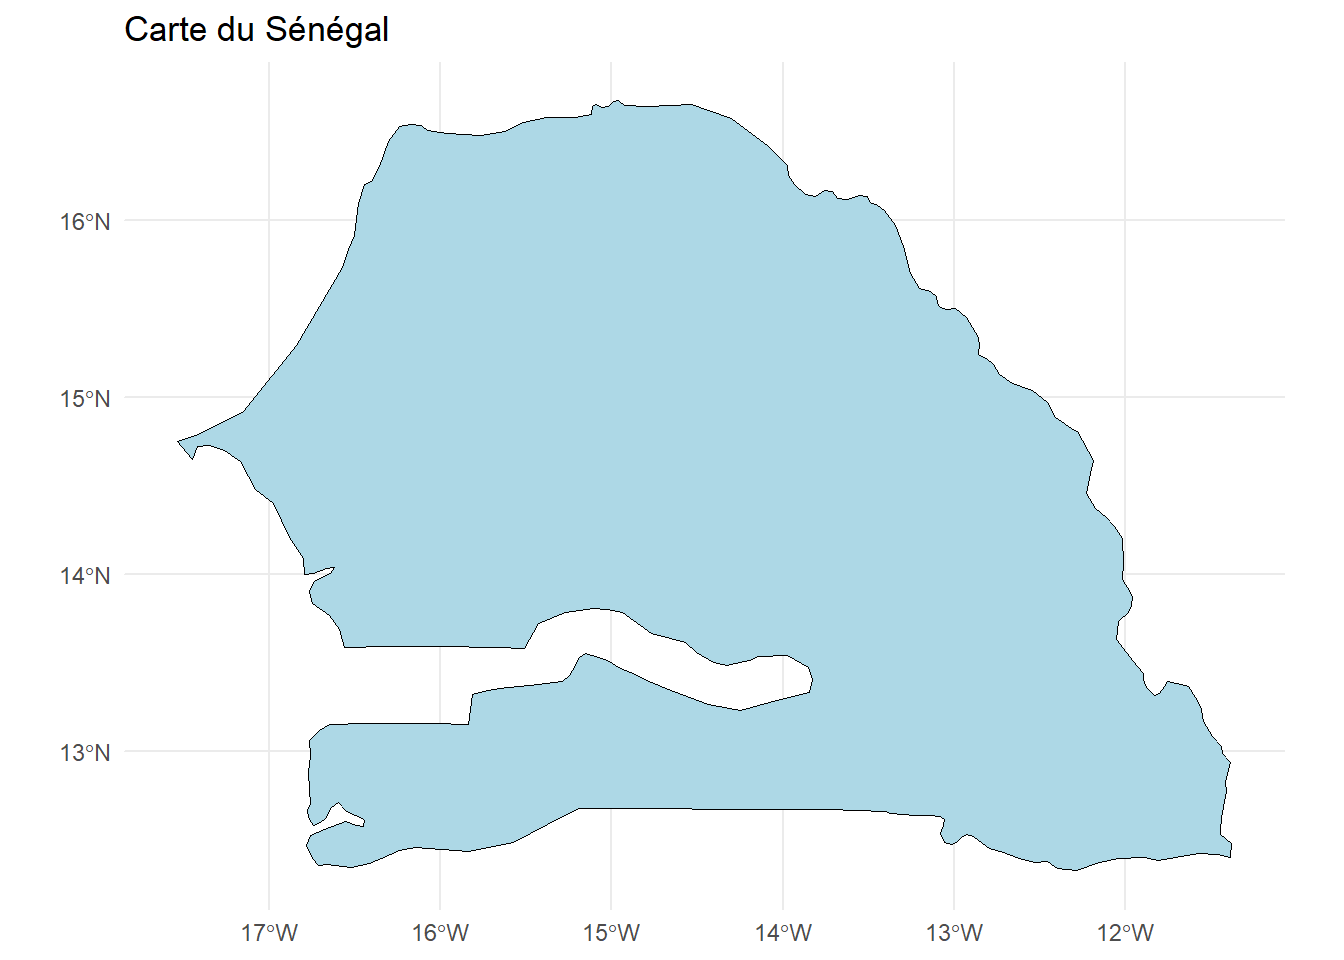
\includegraphics[keepaspectratio]{Stat_Desc_KAFANDO_ILLY_Syntaxe_TP8_files/figure-latex/unnamed-chunk-19-1.pdf}}

\newpage

\section{\texorpdfstring{\textbf{Section 5 : Cartographie par commune
sur les
pays}}{Section 5 : Cartographie par commune sur les pays}}\label{section-5-cartographie-par-commune-sur-les-pays}

\subsection{\texorpdfstring{\emph{Importations des shapefiles
adéquats}}{Importations des shapefiles adéquats}}\label{importations-des-shapefiles-aduxe9quats-2}

Importons les fichiers de subdivision niveau communal

\begin{Shaded}
\begin{Highlighting}[]
\NormalTok{shp\_adm3\_BF }\OtherTok{\textless{}{-}}\NormalTok{ sf}\SpecialCharTok{::}\FunctionTok{st\_read}\NormalTok{(}\StringTok{"../Data/Shapefile/Commune/bfa\_admbnda\_adm3\_igb\_20200323.shp"}\NormalTok{) }\DocumentationTok{\#\# Shapefile delimitant par commune du Burkina}

\NormalTok{shp\_adm3\_SEN }\OtherTok{\textless{}{-}}\NormalTok{ sf}\SpecialCharTok{::}\FunctionTok{st\_read}\NormalTok{(}\StringTok{"../Data/Shapefile/Commune/sen\_admbnda\_adm3\_anat\_20240520.shp"}\NormalTok{) }\DocumentationTok{\#\# Shapefile delimitant par commune du Sénégal}

\NormalTok{shp\_adm3\_NER }\OtherTok{\textless{}{-}}\NormalTok{ sf}\SpecialCharTok{::}\FunctionTok{st\_read}\NormalTok{(}\StringTok{"../Data/Shapefile/Commune/geoBoundaries{-}NER{-}ADM3.shp"}\NormalTok{) }\DocumentationTok{\#\# Shapefile delimitant par commune du Niger}

\NormalTok{shp\_adm3\_BN }\OtherTok{\textless{}{-}}\NormalTok{ sf}\SpecialCharTok{::}\FunctionTok{st\_read}\NormalTok{(}\StringTok{"../Data/Shapefile/Commune/geoBoundaries{-}BEN{-}ADM3.shp"}\NormalTok{) }\DocumentationTok{\#\# Shapefile delimitant par commune du Bénin}
\end{Highlighting}
\end{Shaded}

\subsection{\texorpdfstring{\emph{Quelques
cartes}}{Quelques cartes}}\label{quelques-cartes-2}

\textbf{Dans cette partie, nous ferons des cartes interractives, il est
donc important de savoir ce que c'est.}

\subsubsection{\texorpdfstring{\emph{1.
Définition}}{1. Définition}}\label{duxe9finition}

Les cartes interactives sont des outils puissants permettant de
visualiser et d'explorer des données géographiques de manière dynamique.
Contrairement aux cartes statiques qui affichent une image fixe, les
cartes interactives offrent des fonctionnalités avancées telles que le
\textbf{zoom}, le \textbf{déplacement}, l'\textbf{affichage de pop-ups
d'informations}, et la \textbf{personnalisation des styles en temps
réel}.

\subsubsection{\texorpdfstring{\emph{2. Avantages des Cartes
Interactives}}{2. Avantages des Cartes Interactives}}\label{avantages-des-cartes-interactives}

Les cartes interactives présentent plusieurs avantages par rapport aux
cartes statiques :

\begin{itemize}
\tightlist
\item
  \textbf{Navigation dynamique} : Possibilité de zoomer et de se
  déplacer dans la carte.
\item
  \textbf{Affichage d'informations supplémentaires} : Des pop-ups
  interactifs permettent d'afficher des détails en cliquant sur une
  zone.
\item
  \textbf{Mise à jour en temps réel} : Possibilité d'intégrer des
  données dynamiques ou des flux en direct.
\item
  \textbf{Personnalisation avancée} : L'utilisateur peut activer ou
  désactiver des couches de données pour mieux explorer les
  informations.
\item
  \textbf{Meilleure lisibilité} : Les cartes interactives permettent
  d'adapter l'affichage en fonction du niveau de zoom, évitant ainsi la
  surcharge d'informations.
\end{itemize}

Sur \textbf{R}, nous pouvons utiliser les packages \emph{tmap},
\emph{leaflet} pour sa réalisation.

\textbf{NB : Dans la suite du travail, pour voir les graphiques, il
faudra voir sur la sortie html, car seul cette derniere permet de
visualiser les cartes interractives. La sortie en pdf ne le permet pas.}

\subsubsection{\texorpdfstring{\emph{3. Carte du Burkina suivant les
communes}}{3. Carte du Burkina suivant les communes}}\label{carte-du-burkina-suivant-les-communes}

Nous traçon une carte du Burkina avec des subdivision niveau communal

\begin{Shaded}
\begin{Highlighting}[]
\CommentTok{\# Activer le mode interactif}
\NormalTok{tmap}\SpecialCharTok{::}\FunctionTok{tmap\_mode}\NormalTok{(}\StringTok{"view"}\NormalTok{)}

\NormalTok{tmap}\SpecialCharTok{::}\FunctionTok{tm\_shape}\NormalTok{(shp\_adm3\_BF) }\SpecialCharTok{+} \CommentTok{\# presente la carte avec les limites niveau communes}
  
  \FunctionTok{tm\_polygons}\NormalTok{(}\StringTok{"ADM1\_FR"}\NormalTok{, }\CommentTok{\#Ajoute des couleurs en fonction des régions}
              
             \AttributeTok{popup.vars =} \FunctionTok{setNames}\NormalTok{(}\FunctionTok{c}\NormalTok{(}\StringTok{"ADM3\_FR"}\NormalTok{, }\StringTok{"ADM2\_FR"}\NormalTok{, }\StringTok{"ADM1\_FR"}\NormalTok{), }\CommentTok{\# Specifie les informations visible au clic }
                                    \FunctionTok{c}\NormalTok{(}\StringTok{"Commune"}\NormalTok{, }\StringTok{"Province"}\NormalTok{, }\StringTok{"Région"}\NormalTok{)), }\CommentTok{\# Renomme les elements en nom comprehensible}
              \AttributeTok{border.col =} \StringTok{"black"}\NormalTok{) }\SpecialCharTok{+} \CommentTok{\# couleur des tracées}
  
  \FunctionTok{tm\_text}\NormalTok{(}\StringTok{"ADM3\_FR"}\NormalTok{, }\AttributeTok{size =} \FloatTok{0.8}\NormalTok{, }\AttributeTok{col =} \StringTok{"black"}\NormalTok{, }\AttributeTok{auto.placement =} \ConstantTok{TRUE}\NormalTok{)   }\CommentTok{\# Affiche les noms des communes}
\end{Highlighting}
\end{Shaded}

\subsubsection{\texorpdfstring{\emph{4. Carte du Niger suivant les
communes}}{4. Carte du Niger suivant les communes}}\label{carte-du-niger-suivant-les-communes}

Nous traçon une carte du Niger avec des subdivision niveau communal et
presentant chaque ménage enqueté.

Pour se faire nous devons d'abord transformer la base ménage en objet sf
pour pouvoir representer chaque menage sur la carte.

\begin{Shaded}
\begin{Highlighting}[]
\CommentTok{\# Convertir la base ménage en objet sf (Système de coordonnées WGS84)}

\NormalTok{menages\_sf }\OtherTok{\textless{}{-}} \FunctionTok{st\_as\_sf}\NormalTok{(EHCVM\_Niger, }\AttributeTok{coords =} \FunctionTok{c}\NormalTok{(}\StringTok{"GPS\_\_Longitude"}\NormalTok{, }\StringTok{"GPS\_\_Latitude"}\NormalTok{), }\AttributeTok{crs =} \DecValTok{4326}\NormalTok{)}
\end{Highlighting}
\end{Shaded}

L'affichage des noms sur la carte est bloqué par la bibliothèque
\emph{s2} du package \emph{sf}, pour certaines erreurs de géométrie,
donc désactivons le temporairement afin de pouvoir afficher les
communes.

\begin{Shaded}
\begin{Highlighting}[]
\NormalTok{sf}\SpecialCharTok{::}\FunctionTok{sf\_use\_s2}\NormalTok{(}\ConstantTok{FALSE}\NormalTok{) }
\end{Highlighting}
\end{Shaded}

Maintenant, traçons la carte et superposons les ménages

\begin{Shaded}
\begin{Highlighting}[]
\CommentTok{\# Activer le mode interactif}
\NormalTok{tmap}\SpecialCharTok{::}\FunctionTok{tmap\_mode}\NormalTok{(}\StringTok{"view"}\NormalTok{)}

\CommentTok{\# Créer la carte avec les communes et les ménages}

\FunctionTok{tm\_shape}\NormalTok{(shp\_adm3\_NER)}\SpecialCharTok{+} \CommentTok{\# Tracer la carte du Niger}
  
  \FunctionTok{tm\_polygons}\NormalTok{(}\AttributeTok{fill =} \StringTok{"lightblue"}\NormalTok{) }\SpecialCharTok{+} \CommentTok{\# mettre un fond de couleur bleu clair}

  \FunctionTok{tm\_text}\NormalTok{(}\StringTok{"shapeName"}\NormalTok{, }\AttributeTok{size =} \FloatTok{0.8}\NormalTok{, }\AttributeTok{col =} \StringTok{"black"}\NormalTok{, }\AttributeTok{auto.placement =} \ConstantTok{TRUE}\NormalTok{)}\SpecialCharTok{+}  \CommentTok{\# Affiche les noms des communes}
  
\FunctionTok{tm\_shape}\NormalTok{(menages\_sf) }\SpecialCharTok{+} \CommentTok{\# tracer une autre carte avec des menage, superposer à la premiere}
  
  \FunctionTok{tm\_dots}\NormalTok{(}\AttributeTok{fill =} \StringTok{"pink"}\NormalTok{, }\AttributeTok{size =} \FloatTok{0.5}\NormalTok{, }\CommentTok{\# Representer chaque ménage par un point de couleur rose}
          \AttributeTok{popup.vars =} \FunctionTok{setNames}\NormalTok{(}\FunctionTok{c}\NormalTok{(}\StringTok{"s00q01"}\NormalTok{,}\StringTok{"s00q04"}\NormalTok{, }\StringTok{"s00q05"}\NormalTok{,}\StringTok{"AREA\_SQKM"}\NormalTok{), }
                                \FunctionTok{c}\NormalTok{(}\StringTok{"Région"}\NormalTok{,}\StringTok{"Milieu de résidence"}\NormalTok{, }\StringTok{"Village/Quartier"}\NormalTok{,}\StringTok{"Superficie de la région"}\NormalTok{))) }
\end{Highlighting}
\end{Shaded}

\newpage

\section{\texorpdfstring{\textbf{Conclusion}}{Conclusion}}\label{conclusion}

Grâce à \textbf{R}, il est possible de réaliser des cartes précises et
informatives en utilisant des \textbf{Shapefiles} et les packages
\texttt{sf} et \texttt{ggplot2}. En combinant des données statistiques
et spatiales, nous pouvons explorer de nouvelles perspectives
analytiques et mieux comprendre les dynamiques territoriales.

\end{document}
